\documentclass{beamer}
\usepackage{algorithm}
\usepackage{algorithmic}
\usepackage{listings}
\usepackage{xcolor}
\usepackage{color}

\usepackage[absolute,overlay]{textpos}
\usepackage{graphicx}

\DeclareMathOperator{\sgn}{sgn}

\newcommand{\hilight}[1]{\setlength{\fboxsep}{0pt}\colorbox{yellow}{#1}}


\lstset{basicstyle=\scriptsize\ttfamily,breaklines=true}
\lstset{framextopmargin=50pt}

\usetheme{Warsaw}

\begin{document}

\title{On Second Order Methods in Stochastic Optimization}
\author{Stefan S.}

\begin{frame}
	\titlepage
\end{frame}	

\begin{frame}
	\frametitle{Outline}
	\begin{itemize}
		\pause
		\item Observations about using second order information in smooth stochastic optimization
		\pause
		\item An second order method for L1-regularized optimization with convergence rate and computational compelxity analysis
	\end{itemize}
\end{frame}	


\begin{frame}
	\frametitle{Problem - Minimize Expected Value}
	\[
		\min_{\theta \in \mathbb{R}^n} F(\theta) = \mathbb{E}_z[ f(\theta,z)]
	\]
	\begin{itemize}
		\pause
		\item Optimization procedure updates are performed based on a single sample $\hat{z}$ picked randomly at each iteration
		\pause
		\begin{itemize}
		\item This is the only information we have about the distribution of $z$
		\end{itemize}
		\pause
		\item Have an efficient oracle for evaluating
		\begin{itemize}
		\item $\nabla f(\theta,\hat{z})$
		\end{itemize}
		\pause
		\item Example: Large-scale supervised machine learning
	\end{itemize}
\end{frame}

\begin{frame}
	\frametitle{Stochastic Gradient Method}
	We focus on recursive methods of the form
	\[
		\theta_{t+1}= \theta_t - \alpha_t H_t^{-1} g_t 
	\]
	Where $g_t$ is an unbiased estimate of the true gradient at $\theta_t$
	\begin{itemize}
		\pause
		\item $\alpha_t = \frac{\alpha}{t}$
		\pause
		\item $g_t$ is computed using a single sample
		\pause
		\item Will discuss $H_t^{-1}$ in the following slides
		\begin{itemize}
			\item Murata 1998 analysis suggests that the best choice is $H =\nabla^2 F(\theta^*) $
		\end{itemize} 
	\end{itemize}
\end{frame}

\begin{frame}
	\frametitle{Common Concerns and Ideas}
	\begin{itemize}
		\pause
		\item Batch size selection: reduces variance of gradient estimators
		\begin{itemize}
			\item Instead of using a single sample $\hat{z}$ to compute $g_t=\nabla f(\theta_t,\hat{z})$ \\
			      use sample of size $b$ to compute $g_t=\frac{1}{b}\sum_{i=1}^b \nabla f(\theta_t,z_i)$
		\end{itemize}
		\pause
		\item How to sample $z_t$ (cycle vs random sampling vs shuffling) 
		\pause
		\item Steplength choice - adaptive constant steps (learning rates) work extremely well
		\pause
		\item Aggregated Gradient (Schmidt, Le Roux, and Bach 2013)
		\begin{itemize}
			\item Use $\sum_{i=t-m}^{t} g_i$ instead of the gradient and a constant steplength
			\item SAG 
		\end{itemize}
		\pause
		\item Iterate Averaging
		\begin{itemize}
			\item Bach, Moulines 2013
		\end{itemize}
		\pause
		\item Asymptotically batch methods
		\begin{itemize}
			\item Some methods attempt to work in a batch regime by increasing the batch size as the algorithm progresses (Byrd et. al. 2012, Friedlander et. el 2011)
		\end{itemize}
	\end{itemize}
\end{frame} 

\begin{frame}
	\frametitle{Experimental Evidence: Using a Hessian for $H$ is Good}
		\begin{center}
				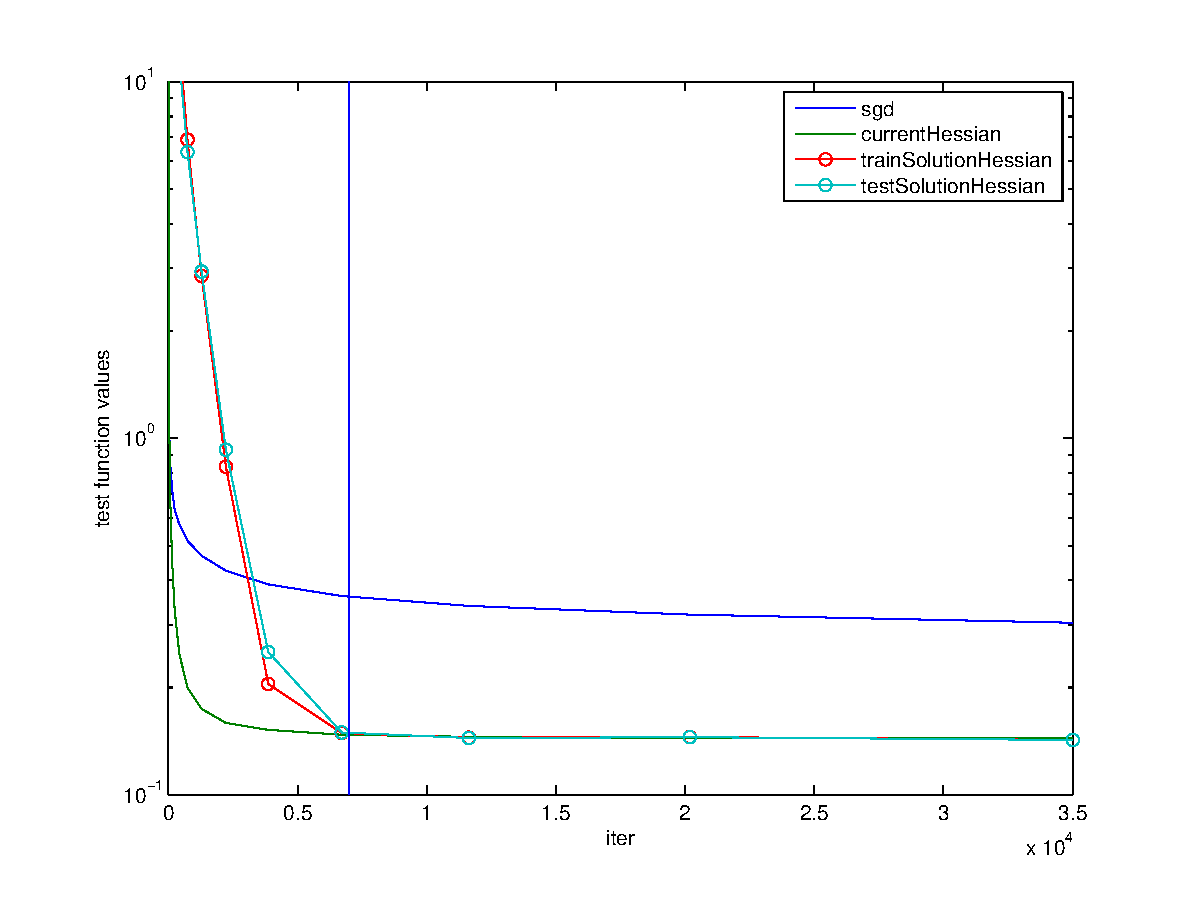
\includegraphics[scale=0.4]{figures/P0.eps}
		\end{center}	
		A random binary logistic regression, with cross-entropy loss. 7000 training data points, 50 variables.
\end{frame}

\begin{frame}
	\frametitle{Conclusion: Approximate the Hessian Matrix}
	\begin{itemize}
		\pause
		\item Approach must be scalable - $O(n)$ operations per iteration, where $n$ is the number of variables
		\pause
		\item Use the Stochastic Quasi-Newton method developed in our group and colleagues (R. Byrd, S. Hansen, J. Nocedal and Y. Singer)
		\pause
		\item Use L-BFGS
		\begin{itemize}
			\item Schraudolph 2007, Mokhtari Ribeiro 2013: Update using noisy gradients from every iteration. They add regularization to deal with noise.
		\end{itemize}
 	\end{itemize}
\end{frame}

\begin{frame}
	\frametitle{SQN Method}
	Idea: Update BFGS approximation more accurately (using a batch larger than 1) but less frequently (to offset the cost)
	\begin{itemize}
		\item Every L iterations compute $s_k = x_i - x_{i-L}$, and an approximation to $y_k = \nabla F(x_i) - \nabla F(x_{i-L}) \approx \nabla^2 f(x_{i-L}) s_k$ \\
		\item Bonus: $s_k^T y_k > 0$ 
	\end{itemize}
	\pause
	Use Limited Memory:
	\begin{itemize}
		\item Bring down update cost and required storage space from $O(n^2)$ to $O(n)$
	\end{itemize}
\end{frame}

\begin{frame}
	\frametitle{SQN Method Outline}
	\begin{algorithmic} [1] 
		\LOOP 
		\IF {$mod(t,L)==0$}
		\STATE $s_k = x_i - x_{i-L}$
		\STATE $y_k = \nabla^2 f(x_{i-L}) s_k$
		\ENDIF
		\STATE Compute $H_t^{-1} g_t$ using two-loop recursion
		\STATE $\theta_{t+1}= \theta_t - \alpha_t H_t^{-1} g_t$ 
		\ENDLOOP 
	\end{algorithmic}
\end{frame}


							 \begin{frame}
\begin{textblock*}{0.2cm}(1.2cm,0.1cm) % {block width} (coords)
							 				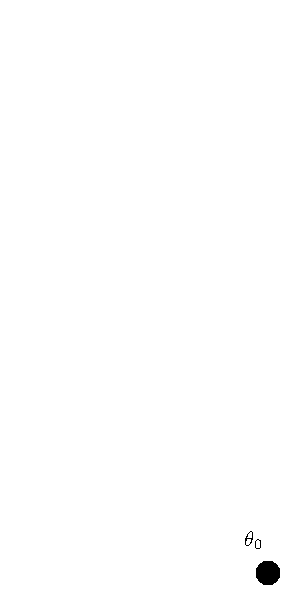
\includegraphics[scale=0.5]{figures/11.eps}
\end{textblock*}
							 \end{frame}

							 \begin{frame}
\begin{textblock*}{0.2cm}(1.2cm,0.1cm) % {block width} (coords)
							 				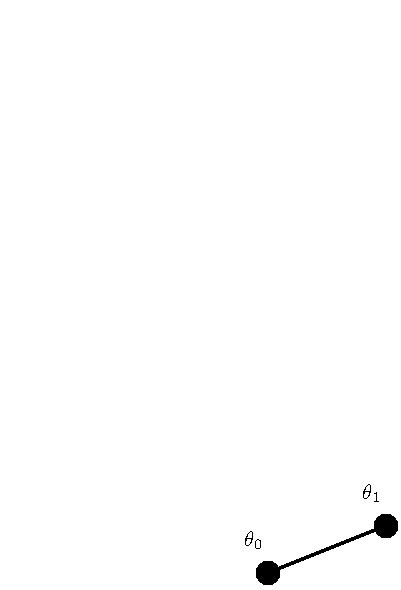
\includegraphics[scale=0.5]{figures/10.eps}
\end{textblock*}
							 \end{frame}
							 \begin{frame}
\begin{textblock*}{0.2cm}(1.2cm,0.1cm) % {block width} (coords)
							 				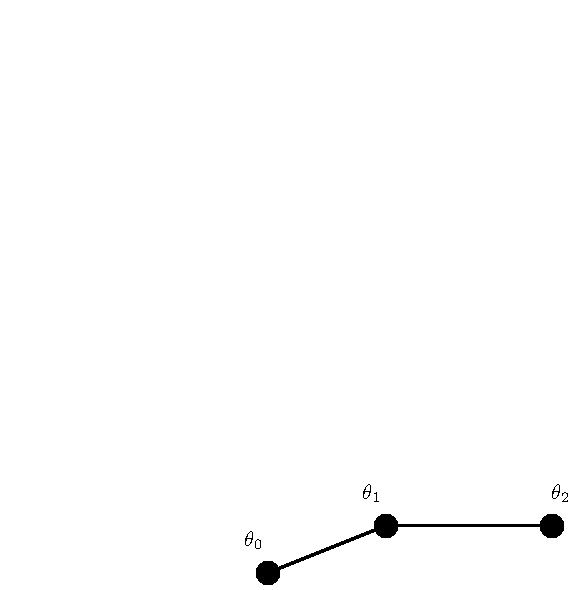
\includegraphics[scale=0.5]{figures/9.eps}
\end{textblock*}
							 \end{frame}
							 \begin{frame}
\begin{textblock*}{0.2cm}(1.2cm,0.1cm) % {block width} (coords)
							 				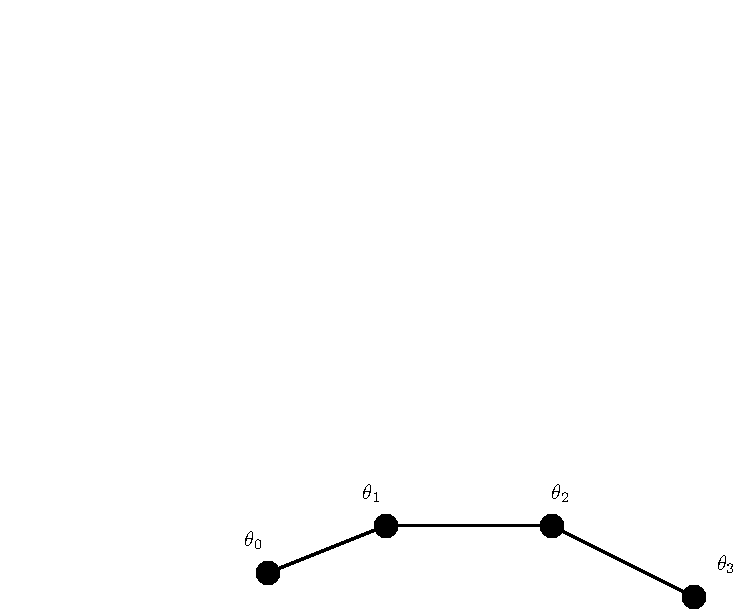
\includegraphics[scale=0.5]{figures/8.eps}
\end{textblock*}
							 \end{frame}
							 \begin{frame}
\begin{textblock*}{0.2cm}(1.2cm,0.1cm) % {block width} (coords)
							 				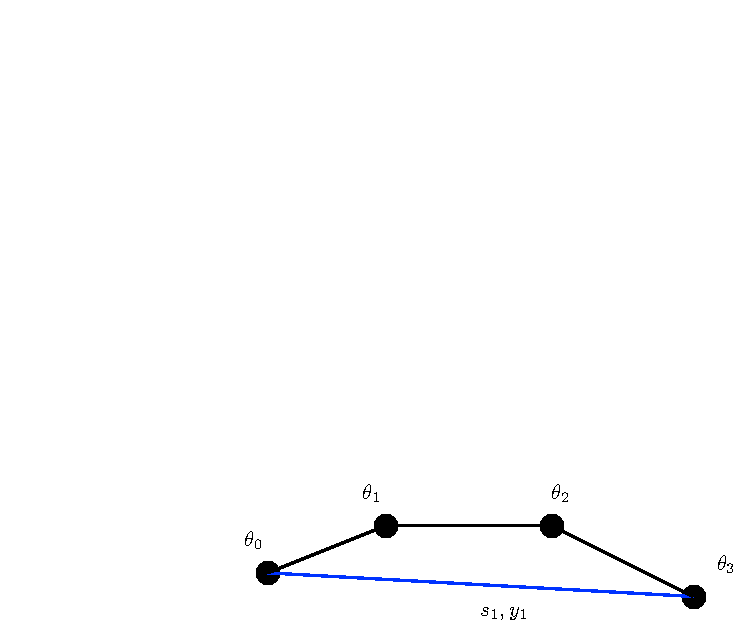
\includegraphics[scale=0.5]{figures/7.eps}
\end{textblock*}
							 \end{frame}
							 \begin{frame}
\begin{textblock*}{0.2cm}(1.2cm,0.1cm) % {block width} (coords)
							 				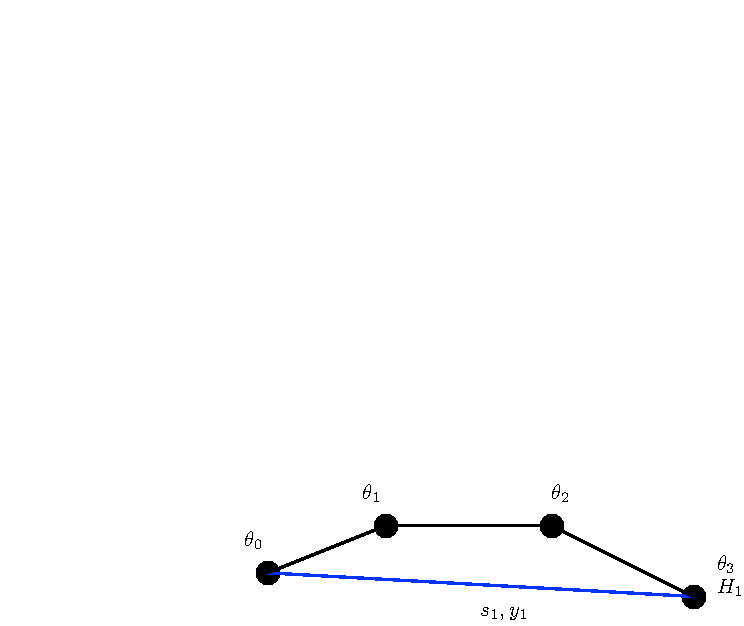
\includegraphics[scale=0.5]{figures/6.eps}
\end{textblock*}
							 \end{frame}
							 \begin{frame}
\begin{textblock*}{0.2cm}(1.2cm,0.1cm) % {block width} (coords)
							 				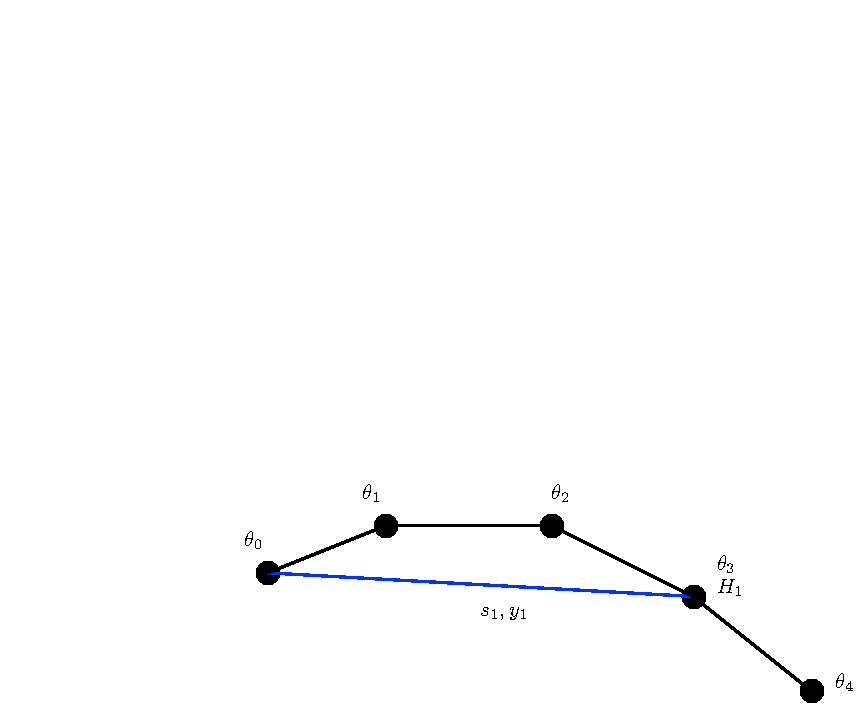
\includegraphics[scale=0.5]{figures/5.eps}
\end{textblock*}
							 \end{frame}
							 \begin{frame}
\begin{textblock*}{0.2cm}(1.2cm,0.1cm) % {block width} (coords)
							 				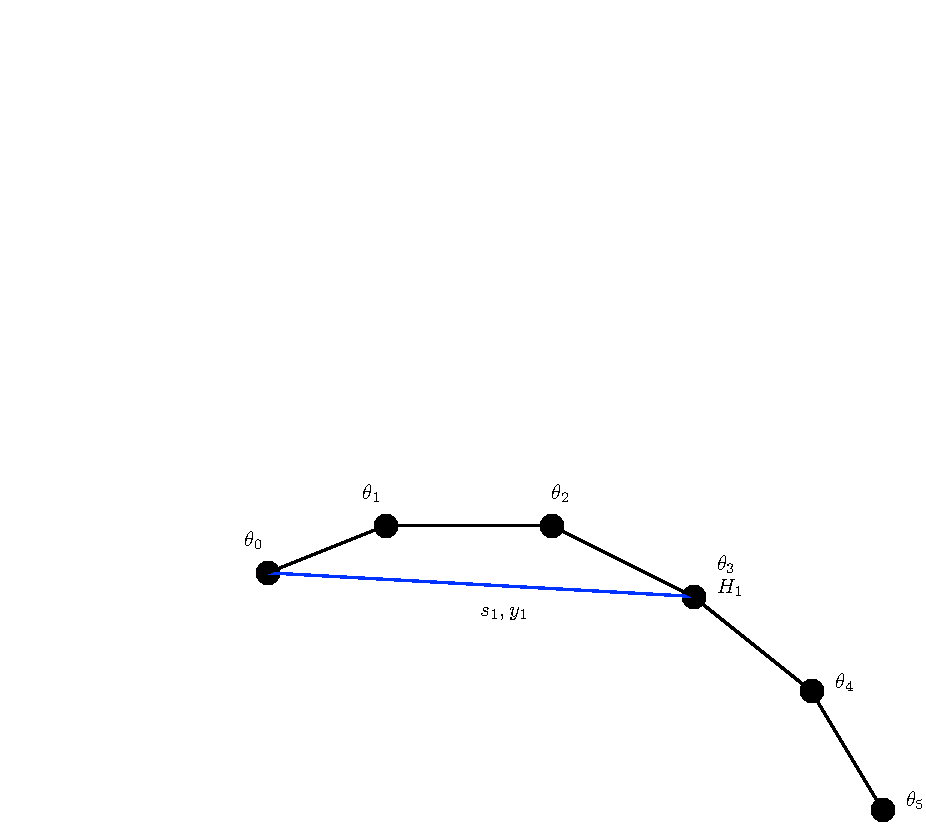
\includegraphics[scale=0.5]{figures/4.eps}
\end{textblock*}
							 \end{frame}
							 \begin{frame}
\begin{textblock*}{0.2cm}(1.2cm,0.1cm) % {block width} (coords)
							 				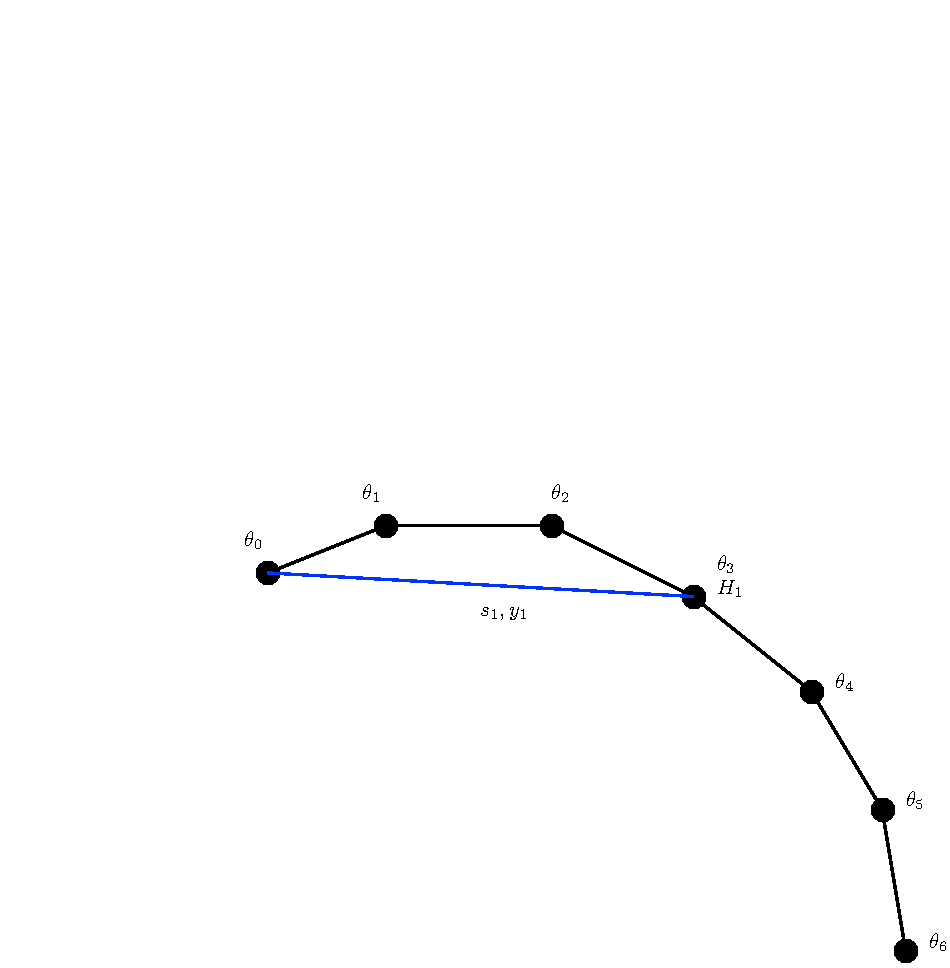
\includegraphics[scale=0.5]{figures/3.eps}
\end{textblock*}
							 \end{frame}
							 \begin{frame}
\begin{textblock*}{0.2cm}(3.15cm,4.15cm) % {block width} (coords)
							 				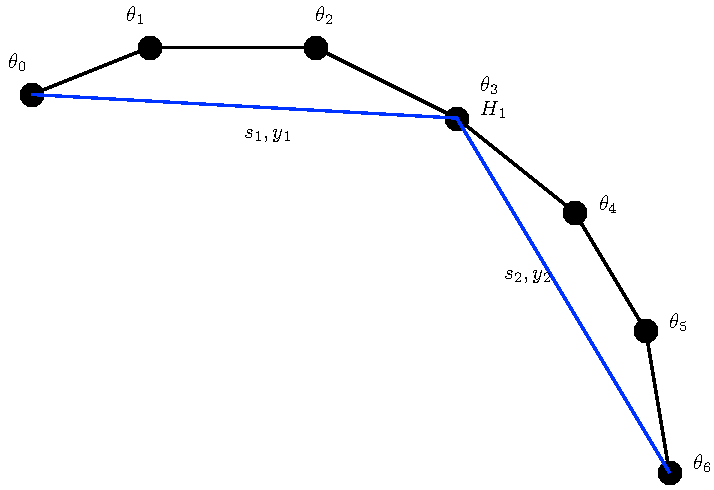
\includegraphics[scale=0.5]{figures/2.eps}
\end{textblock*}
							 \end{frame}
							 \begin{frame}
\begin{textblock*}{0.2cm}(3.15cm,4.15cm) % {block width} (coords)
							 				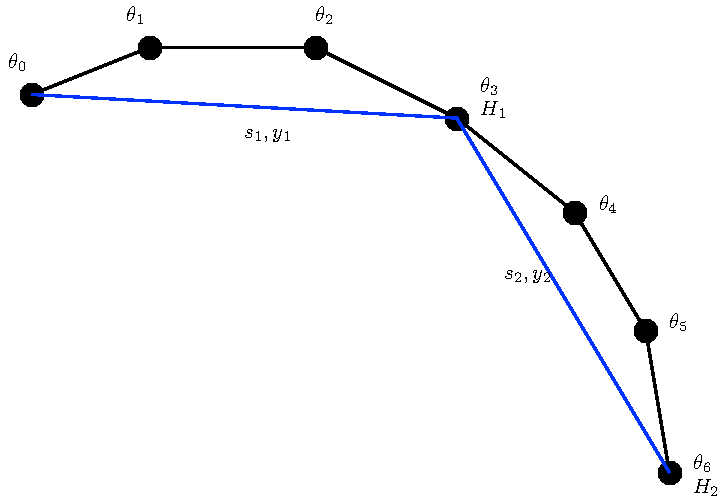
\includegraphics[scale=0.5]{figures/1.eps}
\end{textblock*}
							 \end{frame}
							 
							 
\begin{frame}
	\frametitle{Performance - Random Logistic}
		\begin{center}
				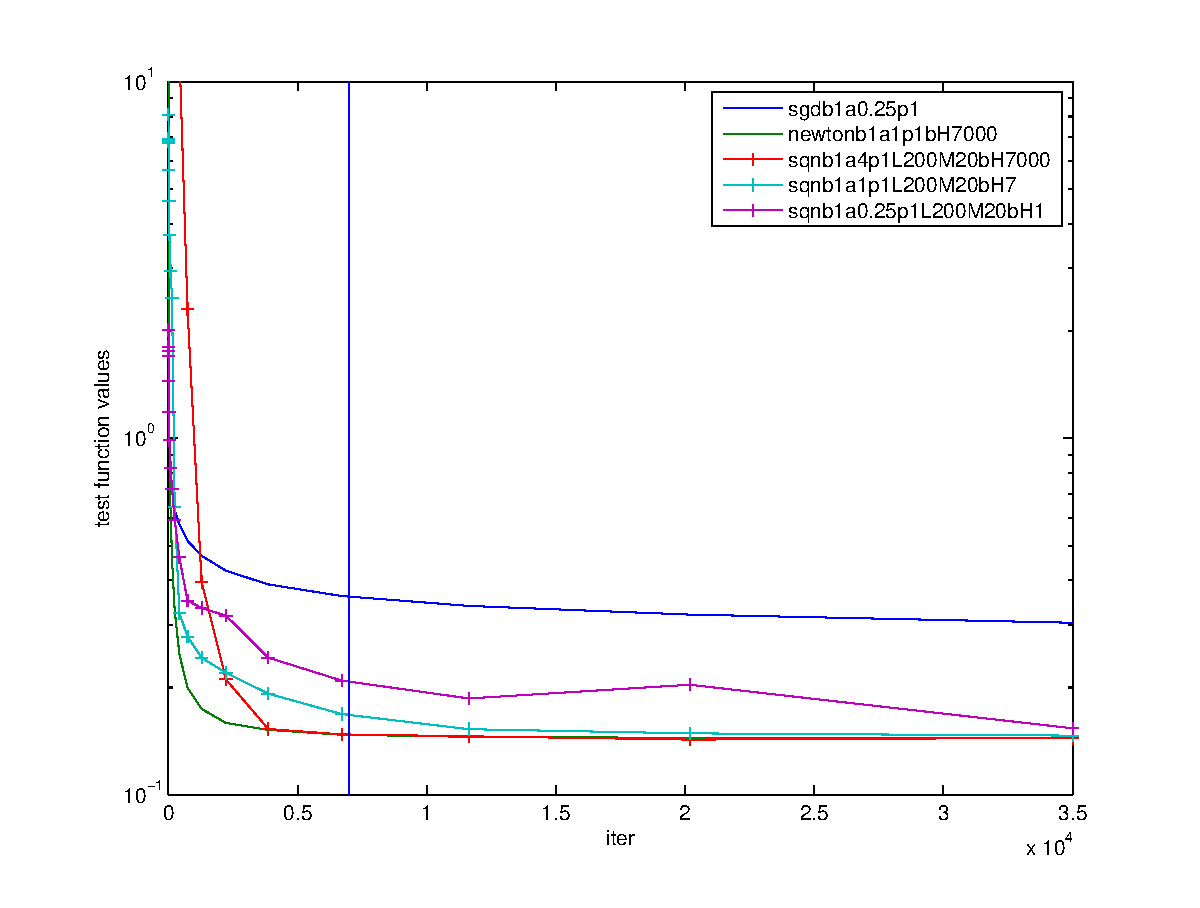
\includegraphics[scale=0.4]{figures/P02.eps}
		\end{center}	
\end{frame}

\begin{frame}
	\frametitle{Why is it promising}
		\begin{center}
				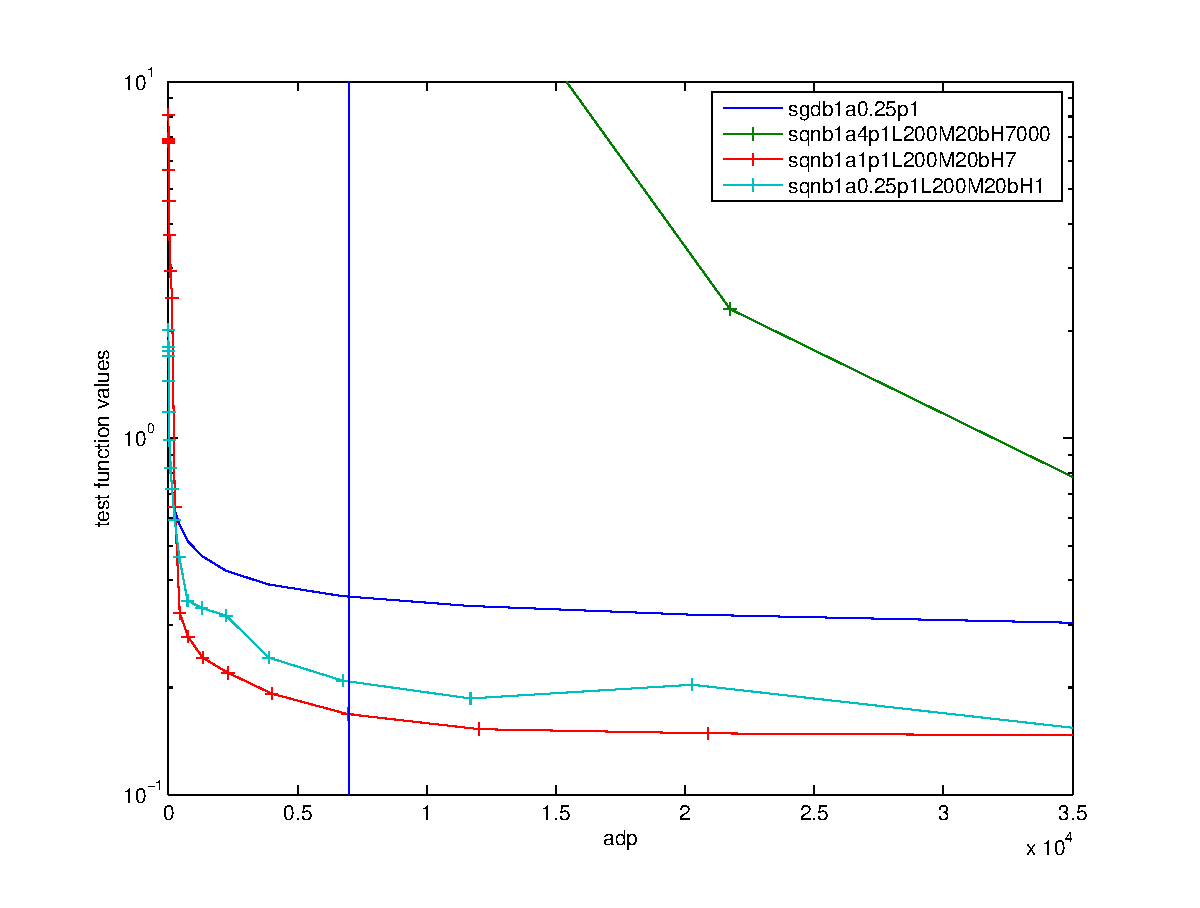
\includegraphics[scale=0.4]{figures/P02b.eps}
		\end{center}	
\end{frame}


\begin{frame}
	\frametitle{This Discussion: Using Gradient Outer Product}
	How about using the estimate $g_k g_k^T$? \\
\pause
		Say the optimization problem is actually
			\[
				\min_{\theta} \frac{1}{m} \sum_{i=1}^{m} f(\langle \theta, \Phi(x_i) \rangle,y_i)]
			\]
			\pause
			The gradient is given by 
			\[
				  \frac{1}{m} \sum_{i=1}^{m} \Phi(x_i) f'(\langle \theta, \Phi(x_i) \rangle,y_i)] = \frac{1}{m} \sum_{i=1}^{m} g_i(\theta)  
			\]
			\pause
			The Hessian is 
			\[
				  \frac{1}{m} \sum_{i=1}^{m} \Phi(x_i)  \Phi(x_i)^T   f''(\langle \theta, \Phi(x_i) \rangle,y_i)] =\frac{1}{m} \sum_{i=1}^{m}  g_i(\theta)g_i^T(\theta) c_i
			\]
	
\end{frame}

\begin{frame}
	\frametitle{Natural Gradient}
	Full Memory: at each iteration
	\begin{align*}
	 H_{t} &= \frac{t-1}{t}G_{t-1} + \frac{1}{t} g_{t-1} g_{t-1}^T \\
	 x_{t+1} &= x_{t} - \alpha_t H_t^{-1} g_t
	\end{align*}
	Update cost $O(n^2)$ \\
	\pause
	Limited Memory: at each iteration
	\begin{align*} 
	 H_{t} &= \frac{1}{K} \sum_{i=t-K}^{t} g_{i} g_{i}^T \\
	 x_{t+1} &= x_{t} - \alpha_t H_t^{-1} g_t
	\end{align*}
	Update cost $O(n)$
\end{frame}

 
\begin{frame}
	\frametitle{AdaGrad}
	Full AdaGrad: at each iteration
	\begin{align*}
	 G_t &= G_{t-1}+ g_t  g_t^T\\
	 H_t &= \delta I + G_t^{1/2}\\
	 x_{t+1} &= x_{t} - \alpha_t H_t^{-1} g_t
	\end{align*}
	Update cost $>>O(n^2)$ \\
	\pause
	Diagonal AdaGrad:  at each iteration
	\begin{align*}
     s_{k,i} &=\sqrt{ ((k-1) s_{k-1,i})^2 +g_{k,i}^2 }, \quad i=1, \cdots, n \\
     H_k &=\delta I + diag(s_k) \\
	 x_{t+1} &= x_{t} - \alpha_t H_t^{-1} g_t
	\end{align*}
	Update cost $O(n)$
\end{frame}

\begin{frame}
	\frametitle{Performance - Random Logistic}
	\begin{center}
	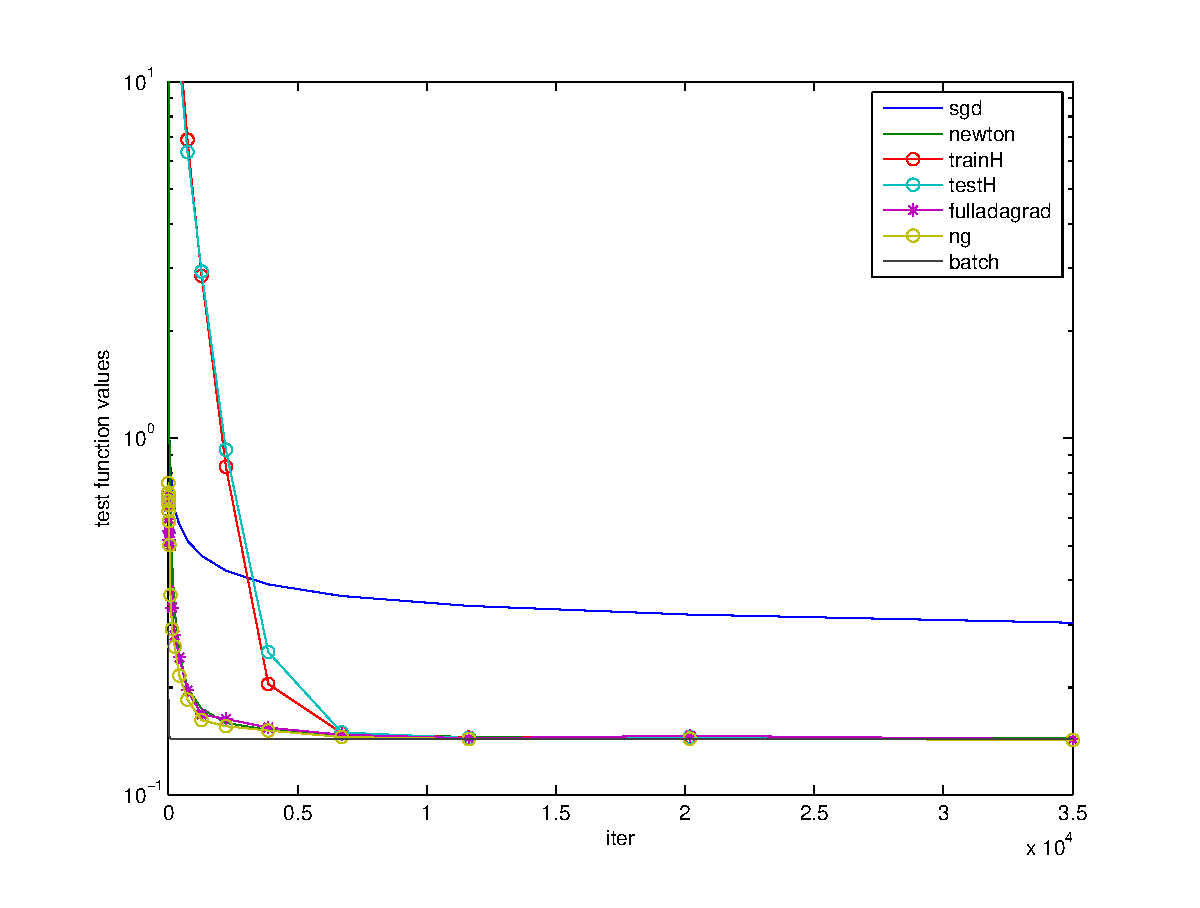
\includegraphics[scale=0.4]{figures/P01.eps}
	\end{center}
	Gradient outer product methods work extremely well
\end{frame}

\begin{frame}
	\frametitle{Test problems}
	RCV1 - binary logistic regression
	\begin{itemize}
		\item 516247 training data points, 112920 variables
	\end{itemize}
	\pause
	A speech recognition dataset - multi-class logistic regression
	\begin{itemize}
		\item 143706 training data points, 30315 variables, 129 classes
	\end{itemize}
	\pause
	A random binary logistic regression problem
	\begin{itemize}
		\item 7000 training data points, 50 variables
		\item A small L2 regularization term 
	\end{itemize}
	\pause
	A random quadratic problem
	\begin{itemize}
		\item 10000 training data points, 20 variables
	\end{itemize}
\end{frame}

\begin{frame}
	\frametitle{Performance - Random Logistic}
	\begin{center}
	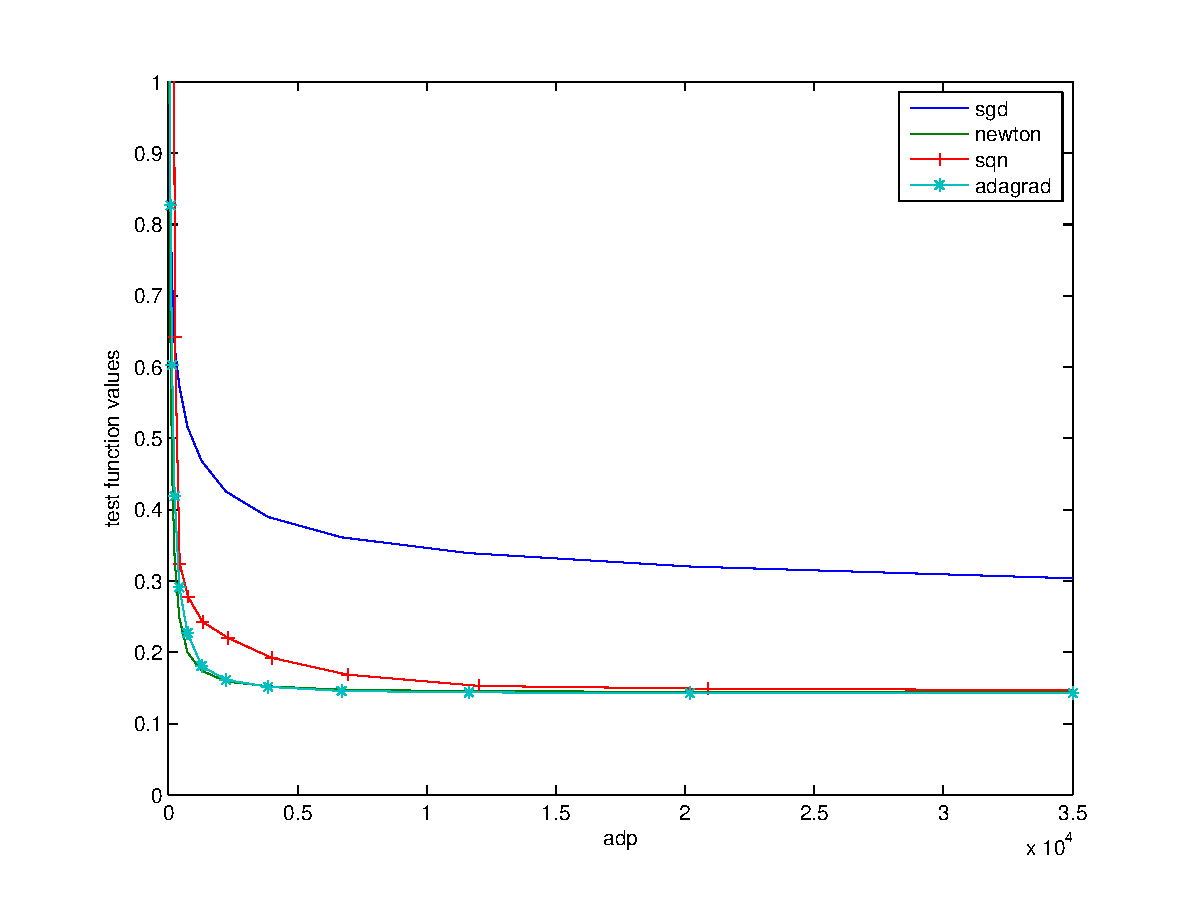
\includegraphics[scale=0.4]{figures/P04.eps}
	\end{center}
\end{frame}

\begin{frame}
	\frametitle{Performance - RCV1}
	\begin{center}
	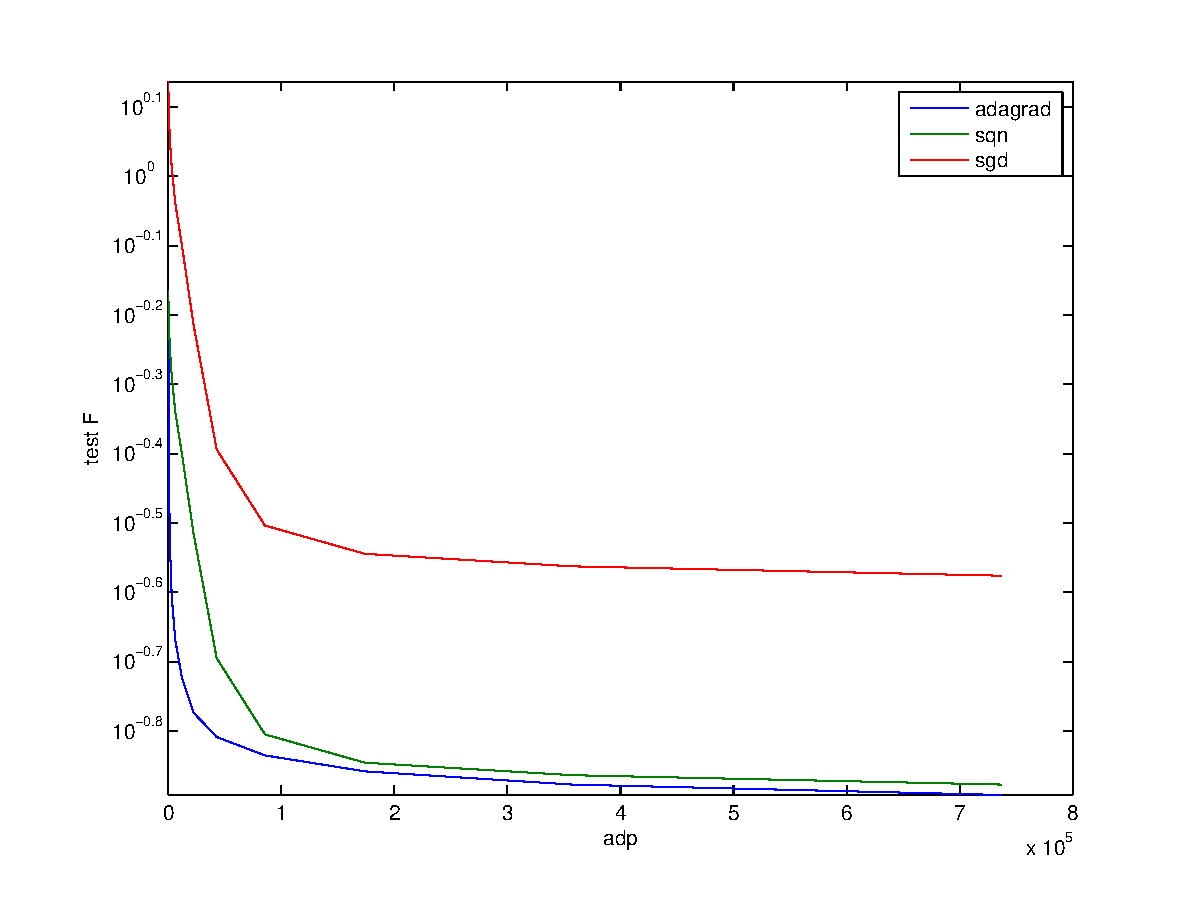
\includegraphics[scale=0.4]{figures/rcv1.eps}
	\end{center}
\end{frame}

\begin{frame}
	\frametitle{Performance - Speech}
	\begin{center}
	\includegraphics[scale=0.4]{figures/speech.eps}
	\end{center}
\end{frame}

\begin{frame}
	\frametitle{Why is our method competetive on some but not other problems?}
	Not all problems of interest are a function of $\langle \theta, \Phi(x)\rangle$.\\
	The multiclass logistic regression has the form
	\[
		F(W) = \frac{1}{N} \sum_{i=1}^N log \left( \frac{exp(W_{z_i} x_i)}{\sum_{j \in C} exp(W_j x_i)} \right)
	\]
\end{frame}

\begin{frame}
	\frametitle{Not All Problems Have This Form!}
	   A random quadratic
	   \[
	   		\min_{\theta}\mathbb{E}_{A,b}[\frac{1}{2}\theta^T A \theta - b^T \theta]
	   \]
	   \begin{itemize}
	   	\item Silly, because averaging samples $A_i$, $b_i$ $i \in {1,\ldots,m}$ can compute full batch gradients in same time as single example gradients
	   	\item Hessian is NOT a multiple of $g g^T$ 
	   \end{itemize}
\end{frame}


							 \begin{frame}
							 	\frametitle{Random Quadratic}
								\begin{center}
							 				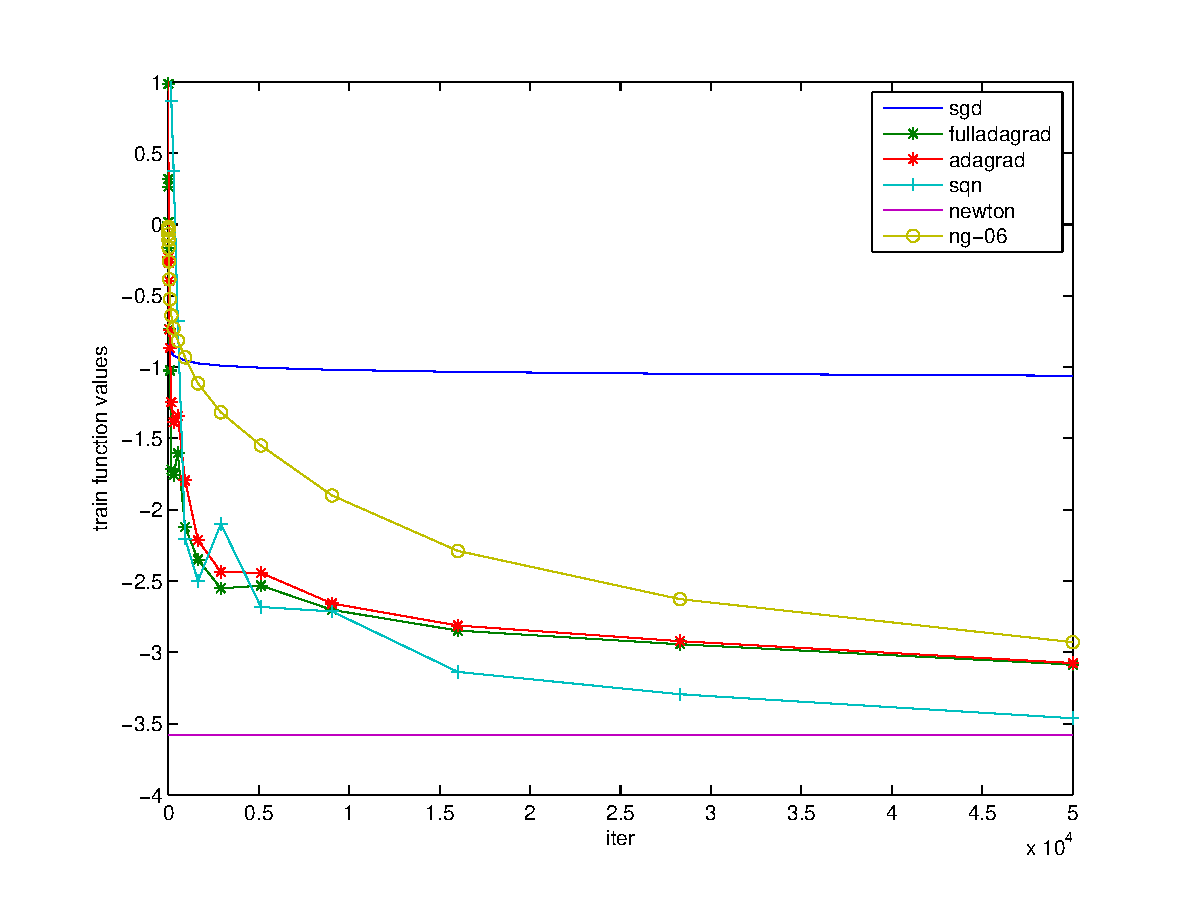
\includegraphics[scale=0.4]{figures/q.eps}
								\end{center}
							 \end{frame}

\begin{frame}
	\frametitle{Conclusions}
	\begin{itemize}
		\item Our method does a good job approximating the action of the Hessian
		\pause
		\begin{itemize}
			\item To Do: test in context of an accelerated method
		\end{itemize} 
		\pause 
		\item Other methods do not outperform putting the true newton matrix. 
		\pause
		\item Success of outer product of gradients more dependent on problem form
	\end{itemize}
\end{frame}


	\begin{frame}
		\frametitle{Beyond SG}
		Averaged SGD - not clear if benefits from second order information\\
		"achieve the same rate of convergence as the optimal unimplementable algorithm" (Polyak, Juditsky 1992)
		\begin{center}
		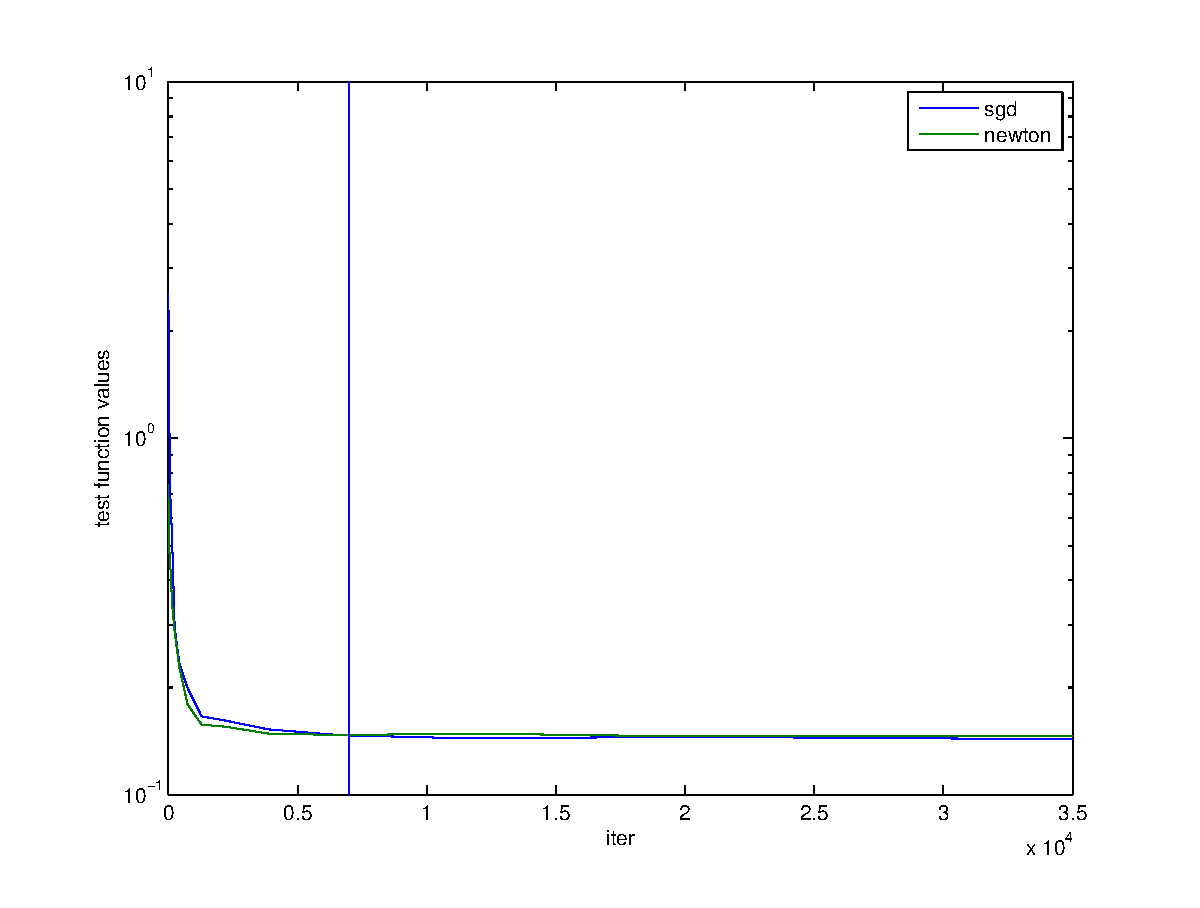
\includegraphics[scale=0.4]{figures/P03.eps}
		\end{center}
	\end{frame}

	\begin{frame}
		\frametitle{Part 2}
		Our motivating problems often have the form 
		\[
			\min_{\theta \in \mathbb{R}^n}  \mathbb{E}_z[ f(\theta,z)] + \tau \|\theta\|_1
		\]
		or
		\[
			\min_{\theta \in \mathbb{R}^n}  F(\theta) + \tau \|\theta\|_1
		\]
		\pause
		Before asking how to approximately use second order information, what relevant methods are there?
	\end{frame}
	

	\begin{frame}
		\frametitle{Deterministic Methods}
		First order methods:
		\begin{itemize}
			\item Proximal Gradient
			\item Accelerated versions
			\item Smoothing  
		\end{itemize}
		\pause
		Second order methods:
		\begin{itemize}
			\item Projected gradient. Two metric projection.
			\item Orthant-Based methods
			\item Block active set 
			\item Interior point
			\item Coordinate Descent?
			\item etc.   
		\end{itemize}
	\end{frame}

	\begin{frame}
		\frametitle{Problem - Quadratic $\ell_1$}
	\begin{equation*}
		\min_{x \in \mathbb{R}^n} \ F(x) = \frac{1}{2}x^T A x - b^T x +\tau \|x\|_1 ,
	\end{equation*}
	We developed an active set algorithm that has 
	\begin{itemize}
		\item A proven convergence rate and a work complexity result
		\item Unusual inexactness criteria for solving the subproblem 
	\end{itemize}
		\end{frame}


\begin{frame}
	\frametitle{Active set: Variables held at 0}
	\begin{center}
			\includegraphics[scale=0.6]{figures/subspace1}
	\end{center}
\end{frame}

\begin{frame}
	\frametitle{Subspace: Smooth $q(x;x^L)$}
		\begin{center}
				\includegraphics[scale=0.6]{figures/subspace2}
		\end{center}	
\end{frame}

\begin{frame}
	\frametitle{Subspace: Unconstrained $q(x;x^L)$ Minimizer}
		\begin{center}
				\includegraphics[scale=0.6]{figures/subspace3}
		\end{center}	
\end{frame}

\begin{frame}
	\frametitle{Subspace: Unconstrained $q(x;x^L)$ Minimizer}
		\begin{center}
				\includegraphics[scale=0.6]{figures/subspace4}
		\end{center}	
\end{frame}

\begin{frame}
	\frametitle{Subspace: Constrained $q(x;x^L)$ Minimizer}
		\begin{center}
				\includegraphics[scale=0.6]{figures/subspace5}
		\end{center}	
\end{frame}

\begin{frame}
	\frametitle{Subspace: $q(x;x^R)$ Minimizer }
		\begin{center}
				\includegraphics[scale=0.6]{figures/subspace6}
		\end{center}	
\end{frame}
           
           
          
                                            
\begin{frame}
\frametitle{Notation}
	\begin{equation*}
		\min_{x \in \mathbb{R}^n} \ F(x) = \frac{1}{2}x^T A x - b^T x +\tau \|x\|_1 ,
	\end{equation*}
We set $v(x) = \omega(x) + \phi(x)$ where
\begin{itemize}
\item $\omega(x) $ contains the components corresponding to $x=0$ \\
\item $\phi(x) $ contains the components corresponding to $x \neq 0$ \\
\end{itemize}


\end{frame} 

\begin{frame}
	\frametitle{$\omega$ and $\phi$}
		\begin{center}
				\includegraphics[scale=0.6]{figures/omegaphi1}
		\end{center}	
\end{frame}


	\begin{frame}
		\frametitle{ISTA-CG}
	\begin{algorithmic}
		[1] \LOOP \STATE $x^{k+1} = \arg \min_y f(x^k) + (y-x^k)^T g(x^k) +\frac{1}{2 \bar{\alpha}^s}\| (y-x^k)\| ^2 + \tau \|y\|_1$
		 \LOOP \IF {$\| \omega(x^k) \| > \| \phi(x^k) \|$} \STATE \textbf{break} \ENDIF \STATE $x^{k+1} = CG(x^k) $
		 \IF { $F(x^{k+1}) > F(x^{k}) - c \| v(x^{k}) \|^2$ } 
		 \STATE \textbf{break} \ENDIF \ENDLOOP \ENDLOOP 
	\end{algorithmic}

	\end{frame}
	


	\begin{frame}
		\frametitle{Modified First Order Step}
		We observed that often the proximal graient step is over-zealous, and releases zero variables too liberally
	\begin{algorithmic}
		[1]\IF {$ \| \omega(x^k) \| \leq \| \phi(x^k) \|$} \STATE $x^{k+1} = \arg \min_y f(x^k) + (y-x^k)^T g^s(x^k) +\frac{1}{2 \bar{\alpha}^s}\| (y-x^k)\| ^2 + \tau \|y\|_1$ \ENDIF \IF {$ \omega(x^k) \| > \| \phi(x^k) \|$} \STATE $\alpha_r = \frac{\omega(x^k)^T \omega(x^k)}{\omega(x^k)^T A\omega(x^k)}$ \STATE $x^{k+1} = x^k - \alpha_r \omega(x^k)$ \ENDIF
	\end{algorithmic}

	\end{frame}
	
	\begin{frame}
		\frametitle{Features of Proposed Method}
		\begin{itemize}
		\item Incorporates second-order information about the function $F$ through an inner conjugate gradient iteration \\
		\pause \item An active set method with a unique termination criteria for the subspace solve \\
		\begin{itemize}
		\item NOT an accuracy criteria. We do not have a pre-defined accuracy which, once reached, terminates the subspace solve.
		\item Automatically solve to high accuracy when a good subproblem is identified. 
		\end{itemize}
		\end{itemize}
	\end{frame}
	

	\begin{frame}
	                                            \frametitle{Convergence: Linear Rate}
	\begin{theorem}
	\label{thm:qlinear} 
	Let $x^{k+1}$ be computed by either a proximal gradient step with $\frac{1}{16L} \leq \bar{\alpha} \leq \frac{1}{L}$, relaxation, or an accepted (not cut back) CG step. Then 
	\begin{equation*}
	F(x^{k+1}) - F^* \leq (1-\frac{\lambda}{16 L}) (F(x^k) - F^*).
	  \end{equation*}
	where $F^*$ is the optimal objective value. 
	\end{theorem}
	                                 \end{frame} 
        
	        \begin{frame}
	                                                    \frametitle{Convergence: Work Complexity}
	      Thus a work complexity result is possible as well. 
	    \begin{corollary}
	    The work complexity (number of matrix vector products) to reach $\epsilon$ accuracy in the objective value is 
	 \begin{equation*}
	  \frac{ 2 \log \{\frac{\epsilon}{(F(x^0) - F^*} \}}{\log\{ \sqrt{1-\frac{\lambda}{16 L}}\} }. 
	   \end{equation*}
	\end{corollary}
	                         \end{frame}
							 
							 
							 

							 \begin{frame}
							 	\frametitle{An example run}
								\begin{center}
							 				\includegraphics[scale=1]{figures/Fig3b.eps}
											\end{center}
							 \end{frame}
							 \begin{frame}
							 	\frametitle{What happened at the end?}
								\begin{center}
							 				\includegraphics[scale=1]{figures/Fig4a.eps}
											\end{center}
							 \end{frame}
							 
							 \begin{frame}
							 	\frametitle{Nearly Quadratic (small regularization parameter)}
								\begin{center}
							 				\includegraphics[scale=1]{figures/Fig4b.eps}
											\end{center}
							 \end{frame}
							 
							 \begin{frame}
							 	\frametitle{Dolan-More Performance Profile: solve to high tolerance}
								\begin{center}
							 				\includegraphics[scale=1]{figures/Fig5b.eps}
											\end{center}
							 \end{frame}
							 \begin{frame}
							 	\frametitle{Efficiency}
								\begin{center}
							 				\includegraphics[scale=1]{figures/Fig7a.eps}
											
											Solved to $tol = 10^{-10}$ within 1 percent of the best method
											\end{center}
							 \end{frame}
							 
							
							 \begin{frame}
							 	\frametitle{Summary}
								\begin{itemize}
									\item Question of inexactness of the second order step was interesting even in the non-stochastic case
									\item Natural stopping criteria exist for the second order step calculations 
								\end{itemize}
							 \end{frame}
							 

							 \begin{frame}
							 				Questions?
							 \end{frame}
							 
							 
							 
							 
							 
\end{document}